

\chapter{Grasping Evaluation Proposal}
\label{cap3:grasping_eval}

After the grasping solution development, researchers encounter a common problem: how to evaluate the proposed methodology? The robotic grasping is typically composed of a complex system that includes, in most cases but not essential, the following issues: object sensing and identification; pose estimation; grasping detection; grasping selection; trajectory planning; force and stability estimation; collision avoidance, among others. All these components have their related error, that can directly affect the grasping performance. For instance, robotic manipulators and 3D sensors have intrinsics action and measurement errors, respectively. Besides, estimation and planning algorithms also have considerable accuracy errors and variations.

Regarding this evaluation shortcoming, some authors proposed well-accepted assessments in the literature. These include point and rectangle grasping representation comparing with distance threshold and Jacquard index in \ac{DL} policies' database ground-truth. The Epsilon and Volume wrench space metrics are also other examples applied to analytical grasping methodologies (Section~\ref{cap2:related_work:sec:grasping_representation}). Although these metrics are focused on a specific grasping step (rectangle and point comparison metric in the detection, and Epsilon and Volume in physical active-pair interaction), they do not reflect the practical robot grasping performance. Some papers specify their own evaluation metric to a robotic grasping in a real scenario, but it is still difficult for readers to have a comparative review of the results. Therefore, these motivations led us to formulate some fair and transparent definitions of the results' assessment. Thus researchers and readers in general can have a clear and fair comparison between different methods found in the literature. With the grasping problem steps presented in Figure~\ref{fig:eval}, it is defined four grasping evaluation success rate criteria: Grasp Prediction, Grasping Reaching, Grasping-Hold, and Handling Grasping.

\begin{figure}[h!] %because of cas-sc
\begin{tcolorbox}
% \centerline{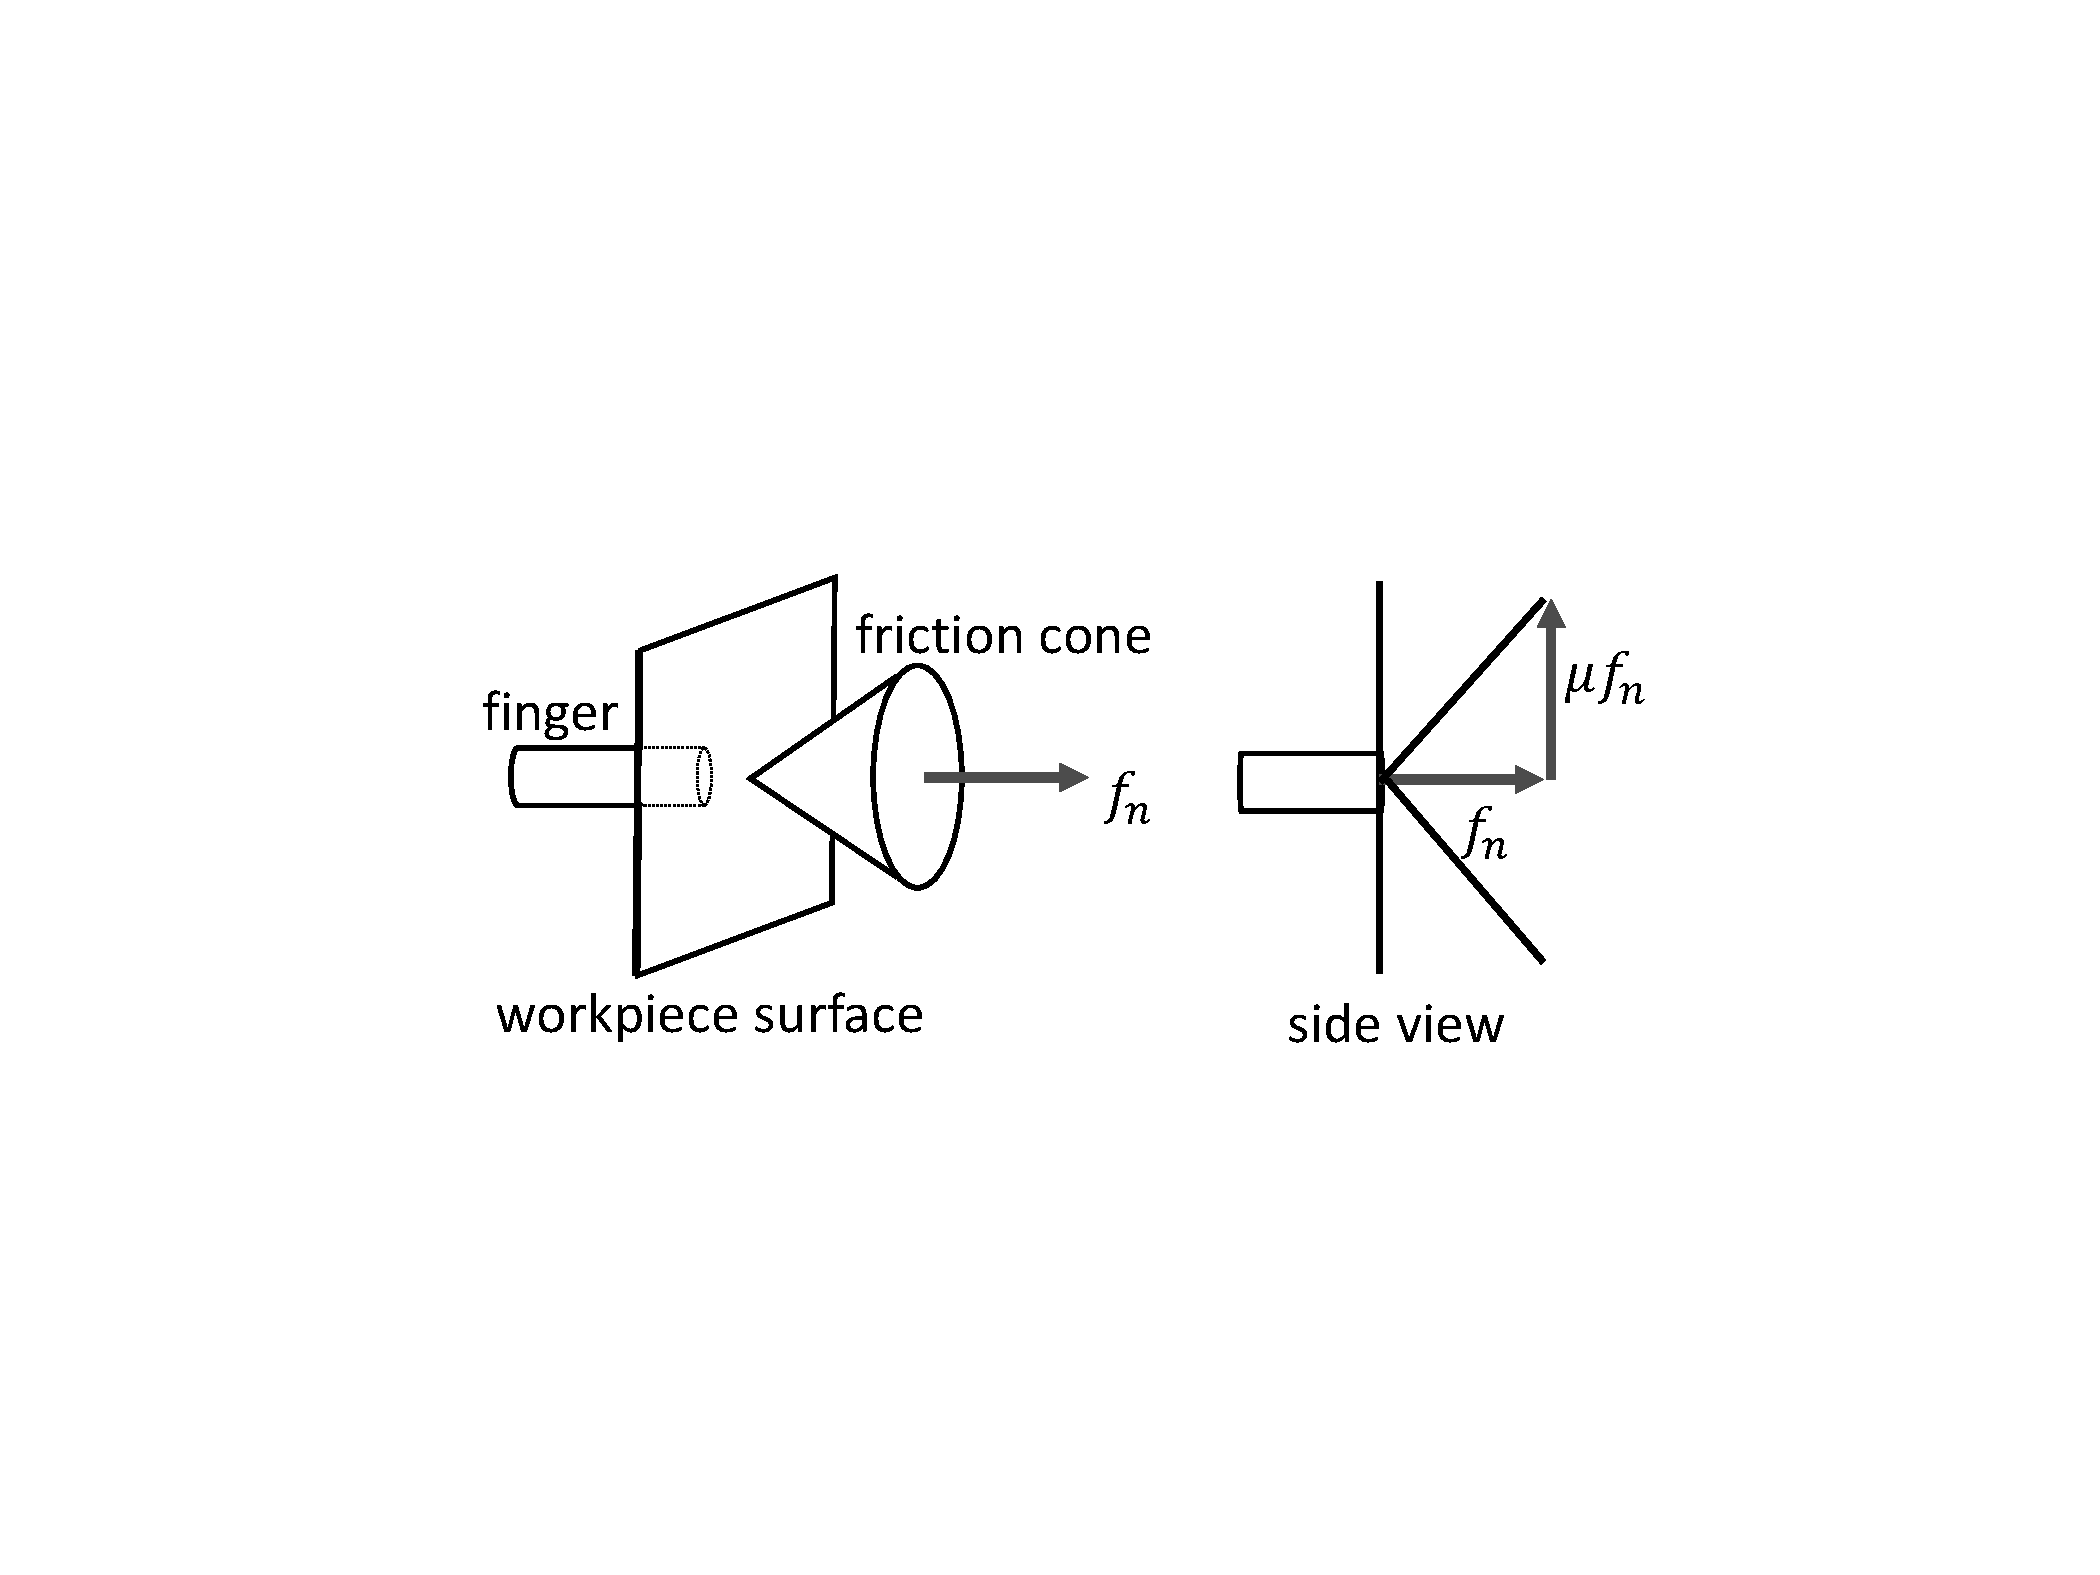
\includegraphics[trim={7cm 8cm 7cm 9cm},clip,width=1\linewidth,angle=0]{Cap2/Figuras/friction_contact.pdf}}
\centerline{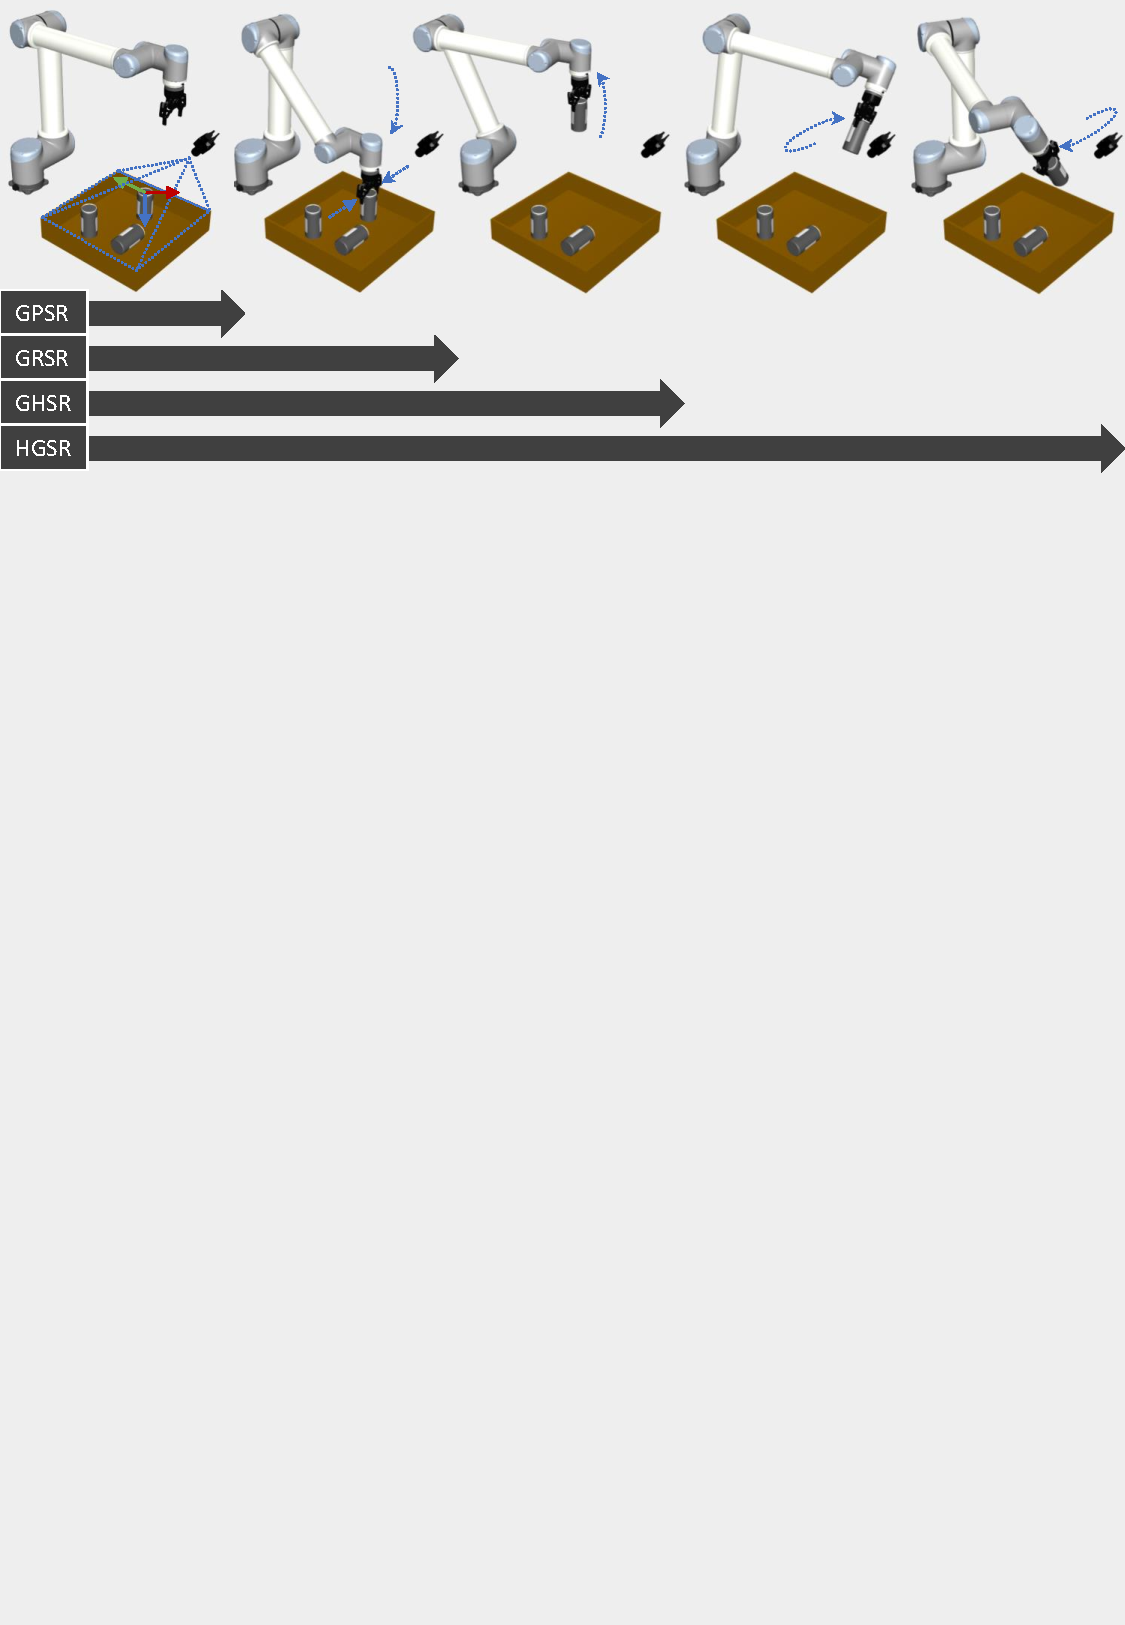
\includegraphics[trim={0cm 19.5cm 0cm 0.07cm},clip,width=1\linewidth,angle=0]{Cap2/Figuras/teste_2.pdf}}
\end{tcolorbox}
\caption{Proposed grasping assessments and their progression timeline. The categories evaluate the grasping performance in different levels based on the complexity of the actions, indicated by the arrows timeline. Each class englobes the prior class resulting in an ascending complexity order from Grasp Prediction (GPSR), Grasping Reaching (GRSR), Grasping-Hold (GHSR) to Handling Grasping success rates (HGSR). The last two successive images describe the 6DOF movements of HGSR.}
\label{fig:eval}
\end{figure}

\section{Grasping Prediction Success Rate}
\label{cap3:grasping_eval:sec:gpsr}

The \ac{GPSR} allows the grasp prediction (or detection) evaluation that consists of the grasp pose estimation generated by methodologies such as the \ac{DL} with \ac{CNN}~\cite{Mahler2019} and the \ac{SANN} optimization technique~\cite{AndrewT2004,carvalho2020}.

In these methods, single or multiple grasping poses are compared with ground-truth and an evaluation of how the grasping estimation is likely to perform, with success, given sensing type: RGB image, Depth map, or Point-Cloud. It is necessary to define if the object is previously known or, in case of \ac{SL} methodologies, if the metric considers sensing-wise (an object sensing data was already presented in the learning phase but with different perspectives from the test case) or object-wise (the object sensing data was never shown in the learning phase) approach. The ground-truth used could be based on a labelled database, such as the \ac{CGD} database, or human supervision considering the user task expertise. Comparison metrics examples are the Euclidean distance between grasping points, the Jacquard threshold to rectangle grasping, the wrench space volume, or the $\epsilon$-value into a simulation procedure. These methods are discussed in Section~\ref{cap2:related_work:sec:grasping_representation}.

This class of success rate is prevalent in deep \ac{CNN} policy proposals, like~\cite{Redmon2015,Kumra2017,asif2018ensemblenet,song2020novel}.Usually, when applied in experimental cases, it has its success rate impaired since it does not evaluate the grasping interaction either the grasping related movements as can be seen in~\cite{Chu2018}.

The processing time related is \ac{GPT}. Normally in this step, the convergence time could be higher in analytical/optimization methods (Section~\ref{cap2:related_work:sec:grasping_approaches:subsec:analytical_review}) demanding a split in grasping planning: offline (\ac{Offline-GPT}) and run-time (\ac{Run-GPT}) approaches~\cite{carvalho2020}. In \ac{DL} policies it could require swap the processing unit from \ac{CPU} to \ac{GPU} generating the \ac{CPU-GPT} and \ac{GPU-GPT}, respectively.

The \ac{CPU-GPT} and \ac{GPU-GPT} could be directly compared; however, the unit processing explicitly shows the hardware requirement. In real applications, an ideally need is the \ac{CPU-GPT}  since \ac{CPU} is cheaper and simpler to be implemented and used, even though this achievement looks like far to state-of-art literature. It is important to note that, with the development of cheaper \acp{GPU} and accessible and straightforward libraries, like CUDA~\cite{cuda}, this could be an irrelevant issue.


\section{Grasping Reaching Success Rate} 
\label{cap3:grasping_eval:sec:grsr}

Suppose a grasping task where sensing is performed, followed by the grasp detection, grasp movement, and gripper's close over the grasp point. In this case, the \ac{GRSR} evaluates the methodology performance considering the deviation from the generate grasping pose and the active grasp point, i.e., the gripper's closing over the object. Therefore, it is a complete way to check the validity of error propagation in a practical scenario compared to \ac{GPSR}, which only evaluates mathematical modelling parameters where practical inconsistencies can appear. This metric includes the accuracy of object sensing, estimation, grasp prediction, grasping acting and can be specified by these error variations. Works like~\cite{moreira_2016} consider this intermediate error assessment, classified as valid or not by a kNN algorithm, critical to a reliable grasping since the \ac{GRSR} defines a starter error that can affect the next task steps.

However, not all physical interactions between the active-pair are evaluated, and only the grasping position precision and friction are appraised. It is important to note that small deviations could generate stable grasps, and a vast number of sensors, robotics manipulators, and grippers have a reduced intrinsic's error. Therefore in a controlled environment, the evaluated error could be small. Also, in referred conditions, the estimation, sensing, and planning algorithms must be designed with caution not to generate high error rates, i.e. a complete error propagation from \ac{GPSR} into \ac{GRSR}. This metric could be useful in precision grasping applications where the contact grasping region is necessary or the grasp slippage avoiding is critical. In addition, the \ac{GRSR} could be considered a filter to eliminate a significant pose grasping error and evaluate its propagation in the overall system.


\section{Grasping-Hold Success Rate} 
\label{cap3:grasping_eval:sec:ghsr}

The \ac{GHSR} allows a complete grasping evaluation criteria. It is considered a robotic grasping application where sensing is performed followed by grasp detection, grasp movement, gripper close over the grasp point, lift the object and hold it for a period. Besides evaluating the error propagation in a practical scenario, as \ac{GRSR} does, it is possible to check the equilibrium of the grasping performance over perturbations and physical interactions, e.g., the slip, wrench space configuration, and the gravity force actuation. This metric could also be evaluated according to object and gripper material friction changes and holding time variation. It important to note that this category excludes the unintentionally grasp that could happen in cluttered and/or bin-picking grasping operations.

\section{Handling Grasping Success Rate}
\label{cap3:grasping_eval:sec:hgsr}

Although \ac{GHSR} could be enough to define a good grasping approach, a more realistic grasping evaluation criteria is the \ac{HGSR}.  Besides including all considerations of \ac{GHSR},  the \ac{HGSR} evaluates the grasping holding of an object and moving it in all robot's DOFs, checking its stability. This metric is relevant for practical scenarios since, in the industry, the work cycle is an important parameter to evaluate. The \ac{GHSR} could be assessed according to the robot movement's speed and acceleration variation, besides the work cycle. It is also possible to include the object's placing movement. However, any analysis of this procedure could confront a new task apart from grasping.

\section{Discussion}
\label{cap3:grasping_eval:sec:discussion}

Aiming to deploy the proposed grasping evaluation in currently state-of-art and stabilising a fair comparison about the literature solutions, Table~\ref{tab:met_state_of_art} presents some grasping approaches and their performance. This table is a guiding tool, and the readers are encouraged to check the source since, besides the specific restriction used in each paper's database that can lead to an unfair comparison, the results presented here are an elucidation give the described conditions: 

\begin{enumerate_jp}
    \item All assessments are restricted to agnostic-grasping (the current challenge in grasping) even though some paper also present better results evaluation with previous knowledge of object shape; 
    \item Only object-wise metric are presented since the object-agnostic is considered;
    \item For tests where the author categorise the objects, the most ``typical'' class is selected in the present table;
    \item The column ``Model Interaction'' indicates if any model interaction is needed to synthesised or selected a grasp (it does not include the database build step of results evaluation) since this affects the grasping performance convergence time;
    \item It is only considered static scenario;
    \item Each methodology was classified according to proposed Grasp Evaluation, Section~\ref{cap3:grasping_eval}. Therefore, if realised, it is presented the most complex category in descending order of: \ac{HGSR}, \ac{GHSR}, \ac{GRSR} and \ac{GPSR}. 
\end{enumerate_jp}


%clutter and isolated scenarios are specified

%%\clear
% Please add the following required packages to your document preamble:
% \usepackage{graphicx}
% \usepackage[table*,xcdraw]{xcolor}
% If you use beamer only pass "xcolor=table*" option, i.e. \documentclass[xcolor=table*]{beamer}


% \usepackage{geometry}
\newgeometry{paper=a4paper,hmargin={1cm,1cm},offset={0cm,-3.5cm}, bottom=-5cm} 

\begin{table*}[h!]
%\vspace{-8.5em}%

\resizebox{0.755\textwidth}{!}{%
\centering
\caption{Object-agnostic grasping methodology proposals and their performances.}
\label{tab:met_state_of_art}
\begin{threeparttable}

\begin{tabular}{cccccccccc}
\hline
\rowcolor[HTML]{C0C0C0} 
%Year &
  \textbf{Methodology Description} &
  \textbf{\begin{tabular}[c]{@{}c@{}}Clutter\\ Scenario\end{tabular}} &
  \textbf{\begin{tabular}[c]{@{}c@{}}Gripper\\ Approach\end{tabular}} &
  \textbf{\begin{tabular}[c]{@{}c@{}}Grasping\\ Representation\end{tabular}} &
  \textbf{\begin{tabular}[c]{@{}c@{}}Model\\ Interaction\end{tabular}} &
  \textbf{\begin{tabular}[c]{@{}c@{}}Sensing\\ data type\end{tabular}} &
  \textbf{\begin{tabular}[c]{@{}c@{}}Processing\\ Time\end{tabular}} &
  \textbf{\begin{tabular}[c]{@{}c@{}}Result\\ Class\end{tabular}} &
  \textbf{\begin{tabular}[c]{@{}c@{}}Performance \\ (Success Grasps)\end{tabular}} \\ \hline
%2004 &
  \begin{tabular}[c]{@{}c@{}}SVM with superquadric \\ shape objects description~\cite{Pelossof2004} \end{tabular}&
  No &
  Generic* &
  Eigengrasp &
  Yes &
  N/R &
  N/R &
  N/R &
  N/R \\
\rowcolor[HTML]{C0C0C0}
%2008 &
  \begin{tabular}[c]{@{}c@{}}Proprietary learning algorithm with\\ logistic regression and image~\cite{Saxena2008}\end{tabular} &
  No &
  Two-Finger &
  Point &
  Yes &
  RGB &
  N/R &
  GHSR &
  87.80\% \\
%2008 &
  \begin{tabular}[c]{@{}c@{}}Proprietary learning algorithm with\\ logistic regression and image~\cite{Saxena2008}\end{tabular} &
  Light &
  Two-Finger &
  Point &
  Yes &
  \begin{tabular}[c]{@{}c@{}}Gray Scale\\ and Depth\end{tabular} &
  N/R &
  HGSR &
  80.00\% \\
\rowcolor[HTML]{C0C0C0} 
%2011 &
  Two-Stage SVM-rank classification~\cite{Jiang2011a} &
  No &
  Two-Finger &
  Rectangle &
  No &
  RGB-D &
  50.000s &
  GHSR &
  87.90\% \\
%2015 &
  Two-stage deep network~\cite{Lenz2015} &
  No &
  Two-Finger &
  Rectangle &
  No &
  RGB-D &
  13.500s &
  GHSR &
  84.00\% \\
\rowcolor[HTML]{C0C0C0} 
%2015 &
  \begin{tabular}[c]{@{}c@{}}Single grasp based on AlexNet\\ direct regression~\cite{Redmon2015}\end{tabular} &
  No &
  Two-Finger &
  Rectangle &
  No &
  RGD &
  0.076s &
  GPSR &
  84.90\% \\
%2015 &
  Multi grasp detection based on AlexNet~\cite{Redmon2015} &
  No &
  Two-Finger &
  Rectangle &
  No &
  RGD &
  0.076s &
  GPSR &
  87.10\% \\
\rowcolor[HTML]{C0C0C0} 
%2016 &
  \begin{tabular}[c]{@{}c@{}}K-NN classification of proprietary dataset and\\ histogram of oriented gradient description~\cite{Pinto2015}\end{tabular} &
  Light &
  Two-Finger &
  Rectangle &
  No &
  RGB-D &
  N/R &
  GPSR &
  69.40\% \\
%2016 &
  \begin{tabular}[c]{@{}c@{}}Linear SVM of proprietary dataset and histogram\\ of oriented gradient description ~\cite{Pinto2015}\end{tabular} &
  Light &
  Two-Finger &
  Rectangle &
  No &
  RGB-D &
  N/R &
  GPSR &
  73.30\% \\
\rowcolor[HTML]{C0C0C0} 
%2016 &
  CNN with proprietary database~\cite{Pinto2015} &
  Light &
  Two-Finger &
  Rectangle &
  No &
  RGB-D &
  N/R &
  GHSR &
  66.00\% \\
%2016 &
  "Common-Sense" analytical heuristic~\cite{Pinto2015} &
  Light &
  Two-Finger &
  Rectangle &
  No &
  RGB-D &
  N/R &
  GPSR &
  62.11\% \\
\rowcolor[HTML]{C0C0C0} 
%2017 &
  \begin{tabular}[c]{@{}c@{}}Unimodal grasp predictor \\ (DCNN + shallow NN)~\cite{Kumra2017}\end{tabular} &
  No &
  Two-Finger &
  Rectangle &
  No &
  RGB or RGD &
  0.062s &
  GPSR &
  88.53\% \\
%2017 &
  \begin{tabular}[c]{@{}c@{}} Multimodal grasp predictor \\ (DCNN + shallow NN)~\cite{Kumra2017} \end{tabular}&
  No &
  Two-Finger &
  Rectangle &
  No &
  \begin{tabular}[c]{@{}c@{}}RGB and\\ 3Channel Depth\end{tabular} &
  0.100s &
  GPSR &
  89.21\% \\
\rowcolor[HTML]{C0C0C0} 
%2017 &
  Image and Tactile DCNN~\cite{Guo2017} &
  No &
  Two-Finger &
  Rectangle &
  No &
  RGB and Tactile &
  N/R &
  GPSR &
  89.10\% \\
%2017 &
  DLSR with NKM-LARS~\cite{Trottier2017} &
  No &
  Two-Finger &
  Rectangle &
  No &
  RGB-D &
  High \tnote{a} &
  GPSR &
  88.07\% \\
\rowcolor[HTML]{C0C0C0} 
%2017 &
  DLSR with GSVQ-ST~\cite{Trottier2017} &
  No &
  Two-Finger &
  Rectangle &
  No &
  RGB-D &
  High \tnote{a} &
  GPSR &
  88.79\% \\
%2017 &
  DLSR with OMP-N~\cite{Trottier2017} &
  No &
  Two-Finger &
  Rectangle &
  No &
  RGB-D &
  High \tnote{a} &
  GPSR &
  88.56\% \\
\rowcolor[HTML]{C0C0C0} 
%2017 &
  DLSR with NKM-N~\cite{Trottier2017} &
  No &
  Two-Finger &
  Rectangle &
  No &
  RGB-D &
  High \tnote{a} &
  GPSR &
  88.17\% \\
%2017 &
  DLSR with RP-N~\cite{Trottier2017} &
  No &
  Two-Finger &
  Rectangle &
  No &
  RGB-D &
  High \tnote{a} &
  GPSR &
  86.61\% \\
\rowcolor[HTML]{C0C0C0} 
%2017 &
  \begin{tabular}[c]{@{}c@{}}CNN classification \\ on analytical designed dataset~\cite{TenPas2017} \end{tabular}&
  Dense &
  Two-Finger &
  \begin{tabular}[c]{@{}c@{}}Analytical\end{tabular} &
  Yes &
  Point Cloud &
  1.000s to 8.000s &
  GHSR &
  89.00\% \\
%2017 &
  Dexnet2.0 and GQ-CNN~\cite{Mahler2017b} &
  No &
  Two-Finger &
  Antipodal  &
  Yes &
  2.5D &
  0.8s &
  HGSR &
  80.00\% \\ %80$\pm$11
\rowcolor[HTML]{C0C0C0} 
%2017 &
  Dexnet2.0 and GQ-CNN~\cite{Mahler2017b} &
  No &
  Two-Finger &
  Antipodal  &
  Yes &
  2.5D &
  0.800s &
  HGSR &
  93.00\% \\ %93$\pm$6\%
%2017 &
  REG~\cite{Mahler2017b} &
  No &
  Two-Finger &
  Antipodal  &
  Yes &
  2.5D &
  2.600s &
  HGSR &
  52.00\% \\ %52$\pm$14
\rowcolor[HTML]{C0C0C0} 
%2017 &
  IGQ~\cite{Mahler2017b} &
  No &
  Two-Finger &
  Antipodal  &
  Yes &
  2.5D &
  1.900s &
  HGSR &
  60.00\% \\%60$\pm$13
%2017 &
  IGQ~\cite{Mahler2017b} &
  No &
  Two-Finger &
  Antipodal  &
  Yes &
  2.5D &
  1.900s &
  HGSR &
  70.00\% \\ %70$\pm$10
\rowcolor[HTML]{C0C0C0} 
%2017 &
  CG-CNN with DexNet 2.1~\cite{Mahler2017d} &
  Dense &
  Two-Finger &
  Antipodal  &
  Yes &
  PointCloud &
  9.400s &
  HGSR &
  85.00\% \\
%2017 &
  CG-CNN with DexNet 2.0~\cite{Mahler2017d} &
  Dense &
  Two-Finger &
  Antipodal  &
  Yes &
  PointCloud &
  10.000s &
  HGSR &
  81.00\% \\
\rowcolor[HTML]{C0C0C0} 
%2017 &
  SVM with geometric descriptions~\cite{Mahler2017d} &
  Dense &
  Two-Finger &
  Antipodal  &
  Yes &
  PointCloud &
  12.857s &
  HGSR &
  64,00\% \\
%2018 &
  \begin{tabular}[c]{@{}c@{}}SVM Classifier based on \\ analytical designed dataset~\cite{tenPas}\end{tabular} &
  No &
  Two-Finger &
  Antipodal  &
  Yes &
  PointCloud & % Registered 2 Views
  N/R &
  HGSR &
  87.80\% \\
\rowcolor[HTML]{C0C0C0} 
%2018 &
  \begin{tabular}[c]{@{}c@{}}SVM Classifier based on \\ analytical designed dataset~\cite{tenPas}\end{tabular} &
  Dense &
  Two-Finger &
  Antipodal  &
  Yes &
  PointCloud & % Registered 2 Views
  N/R &
  HGSR &
  73.00\% \\
%2018 &
  VGG-16 (Single Object - Single Grasp)~\cite{Chu2018} &
  No &
  Two-Finger &
  Rectangle &
  No &
  RGB-D &
  0.058s &
  GPSR &
  91.70\% \\
\rowcolor[HTML]{C0C0C0} 
%2018 &
  RESNET50 (Single Object - Single Grasp)~\cite{Chu2018} &
  No &
  Two-Finger &
  Rectangle &
  No &
  RGB &
  0.120s &
  GPSR &
  95.50\% \\
%2018 &
  RESNET50 (Single Object - Single Grasp)~\cite{Chu2018} &
  No &
  Two-Finger &
  Rectangle &
  No &
  RGBD &
  0.120s &
  GHSR &
  89.00\% \\
\rowcolor[HTML]{C0C0C0} 
%2018 &
  \begin{tabular}[c]{@{}c@{}}EnsembleNet  \\ (MobileNet (Reg.) + VGG16 (Reg.) + ResNet50 (Reg.)) \\ \cite{asif2018ensemblenet}\end{tabular} &
  Light &
  Two-Finger &
  Rectangle &
  No &
  RGB-D &
  N/R &
  GPSR &
  91.20\% \\
%2018 &
  \begin{tabular}[c]{@{}c@{}}EnsembleNet\\ (MobileNet (Joint) + VGG16 (Joint) + ResNet50 (Joint)) \\ \cite{asif2018ensemblenet}\end{tabular} &
  Light &
  Two-Finger &
  Rectangle &
  No &
  RGB-D &
  N/R &
  GPSR &
  93.70\% \\
\rowcolor[HTML]{C0C0C0} 
%2018 &
  \begin{tabular}[c]{@{}c@{}}EnsembleNet \\ (MobileNet (Joint.) + VGG16 (Reg.) + ResNet50 (Joint.)) \\ \cite{asif2018ensemblenet}\end{tabular} &
  Light &
  Two-Finger &
  Rectangle &
  No &
  RGB-D &
  N/R &
  GPSR &
  92.60\% \\
%2018 &
  Planarity Optimization~\cite{Mahler2017} &
  No &
  Suction &
  \begin{tabular}[c]{@{}c@{}}Simple Cup \\      Analytical Model\end{tabular} &
  Yes &
  PointCloud &
  N/R &
  HGSR &
  67.00\% \\
\rowcolor[HTML]{C0C0C0} 
%2018 &
  Centroid Optimization~\cite{Mahler2017} &
  No &
  Suction &
  \begin{tabular}[c]{@{}c@{}}Simple Cup \\      Analytical Model\end{tabular} &
  Yes &
  PointCloud &
  N/R &
  HGSR &
  78.00\% \\
%2018 &
  Planarity and Centroid Optimization~\cite{Mahler2017} &
  No &
  Suction &
  \begin{tabular}[c]{@{}c@{}}Simple Cup \\      Analytical Model\end{tabular} &
  Yes &
  PointCloud &
  N/R &
  HGSR &
  67.00\% \\
\rowcolor[HTML]{C0C0C0} 
%2018 &
  GQ-CNN with Adversarial dataset~\cite{Mahler2017} &
  No &
  Suction &
  \begin{tabular}[c]{@{}c@{}}Simple Cup \\      Analytical Model\end{tabular} &
  Yes &
  PointCloud &
  N/R &
  HGSR &
  67.00\% \\
%2018 &
  \begin{tabular}[c]{@{}c@{}}GQ-CNN with DexNet 3.0 and Adversarial datasets \\~\cite{Mahler2017}\end{tabular} &
  No &
  Suction &
  \begin{tabular}[c]{@{}c@{}}Simple Cup \\      Analytical Model\end{tabular} &
  Yes &
  PointCloud &
  3.000s &
  HGSR &
  82.00\% \\
\rowcolor[HTML]{C0C0C0} 
%2018 &
  \begin{tabular}[c]{@{}c@{}} QG-CNN and DexNet2.0\\~\cite{jaskowski2018improved}\end{tabular} &
  Dense &
  Two-Finger &
  \begin{tabular}[c]{@{}c@{}}Antipodal \\ \end{tabular} &
  Yes &
  PointCloud &
  N/R &
  GPSR &
  86.70\% \\
%2018 &
  FCN and Q-Learning~\cite{Zeng2018} &
  Dense &
  Two-Finger &
  \begin{tabular}[c]{@{}c@{}}Antipodal \\ \end{tabular} &
  Yes &
  Heightmaps &
  N/R &
  GHSR &
  83.30\% \\
\rowcolor[HTML]{C0C0C0} 
%2018 &
  CNN and servoing heuristic~\cite{Levine2018} &
  Dense &
  Two-Finger &
  Analytical &
  No &
  RGB &
  N/R &
  HGSR &
  82.50\% \\
%2019 &
  \begin{tabular}[c]{@{}c@{}}Single grasp based on AlexNet direct regression\\ with Grasp Path description~\cite{Chen2019}\end{tabular} &
  No &
  Two-Finger &
  Rectangle &
  No &
  RGD &
  N/R &
  GPSR &
  81.90\% \\
\rowcolor[HTML]{C0C0C0} 
%2019 &
  \begin{tabular}[c]{@{}c@{}}Multi grasp based on AlexNet direct regression\\ Grasp Path description~\cite{Chen2019}\end{tabular} &
  No &
  Two-Finger &
  Rectangle &
  No &
  RGD &
  N/R &
  GPSR &
  84.70\% \\
%2019 &
  \begin{tabular}[c]{@{}c@{}}Single grasp based on ResFCNN and \\ 2D Belief Map description~\cite{Ghazaei2019}\end{tabular} &
  No &
  Two-Finger &
  2D Belief Map &
  No &
  RGB &
  N/R &
  GPSR &
  81.00\% \\
\rowcolor[HTML]{C0C0C0} 
%2019 &
  \begin{tabular}[c]{@{}c@{}}Multi grasp based on ResFCNN and \\ 2D Belief Map description~\cite{Ghazaei2019}\end{tabular} &
  No &
  Two-Finger &
  2D Belief Map &
  No &
  RGB &
  N/R &
  GPSR &
  90.60\% \\
%2019 &
  6-DOF GraspNet~\cite{Mousavian_2019_ICCV} &
  Light &
  Two-Finger &
  \begin{tabular}[c]{@{}c@{}}Point Cloud\\Shape \end{tabular} &
  Yes &
  PointCloud &
  3.040s &
  GHSR &
  88.00\% \\
\rowcolor[HTML]{C0C0C0} 
%2019 &
  \begin{tabular}[c]{@{}c@{}}Ambidextrous QG-CNN and\\ DexNet4.0~\cite{Mahler2019}\end{tabular} &
  Dense &
  \begin{tabular}[c]{@{}c@{}}Two-Fingers and\\       Suction Cup\end{tabular} &
  \begin{tabular}[c]{@{}c@{}}Antipodal and\\       Analytical Suction\end{tabular} &
  Yes &
  PointCloud &
  11.538s &
  HGSR &
  95.00\% \\
%2019 &
  Suction geometry heuristic~\cite{Mahler2019} &
  Dense &
  \begin{tabular}[c]{@{}c@{}}Two-Fingers and\\       Suction Cup\end{tabular} &
  \begin{tabular}[c]{@{}c@{}}Simple Cup \\      Analytical Model\end{tabular} &
  Yes &
  PointCloud &
  11.842s &
  HGSR &
  80.00\% \\
\rowcolor[HTML]{C0C0C0} 
%2019 &
  \begin{tabular}[c]{@{}c@{}}Composite (Two-Finger and suction) \\ geometric heuristic~\cite{Mahler2019}\end{tabular} &
  Dense &
  \begin{tabular}[c]{@{}c@{}}Two-Fingers and \\      Suction Cup\end{tabular} &
  \begin{tabular}[c]{@{}c@{}}Antipodal and \\ Analytical\end{tabular} &
  Yes &
  PointCloud &
  15.126s &
  HGSR &
  76.00\% \\
%2019 &
  \begin{tabular}[c]{@{}c@{}}Ambidextrous QG-CNN with\\ DexNet2.0 and DexNet 3.0~\cite{Mahler2019}\end{tabular} &
  Dense &
  \begin{tabular}[c]{@{}c@{}}Two-Fingers and\\ Suction Cup\end{tabular} &
  \begin{tabular}[c]{@{}c@{}}Antipodal and\\ Analytical\end{tabular} &
  Yes &
  PointCloud &
  14.117s &
  HGSR &
  76.00\% \\
\rowcolor[HTML]{C0C0C0} 
%2019 &
  FCN and ConvNet~\cite{Zeng2019} &
  Dense &
  \begin{tabular}[c]{@{}c@{}}Two-Fingers and \\ Suction Cup\end{tabular} &
  \begin{tabular}[c]{@{}c@{}}Discrete Set of\\  Primitives Grasps\end{tabular} &
  Yes &
  RGB-D &
  N/R &
  HGSR &
  \begin{tabular}[c]{@{}c@{}}92.40\% (Suction) \\ 96.70\% (Gripper)\end{tabular} \\
%2019 &
  \begin{tabular}[c]{@{}c@{}}Suction heuristic based on surface normal \\ variance over a cloud~\cite{Zeng2019}\end{tabular} &
  Dense &
  Suction Cup &
  \begin{tabular}[c]{@{}c@{}}Simple Cup \\      Analytical model\end{tabular} &
  Yes &
  PointCloud &
  N/R &
  HGSR &
  35.20\% \\
\rowcolor[HTML]{C0C0C0} 
%2019 &
  \begin{tabular}[c]{@{}c@{}}Antipodal heuristic in hill \\ format shapes cloud~\cite{Zeng2019}\end{tabular} &
  Dense &
  Two-Finger &
  Antipodal  &
  Yes &
  PointCloud &
  N/R &
  HGSR &
  92.50\% \\
%2020 &
  \begin{tabular}[c]{@{}c@{}}Backboned in Blacknet53 (YOLOv3) \\ with Grasp Path description~\cite{Chen2020}\end{tabular} &
  No &
  Two-Finger &
  Rectangle &
  No &
  RGB &
  0.110s &
  GPSR &
  94.60\% \\
\rowcolor[HTML]{C0C0C0} 
%2020 &
  One stage region convolutional network~\cite{song2020novel} &
  No &
  Two-Finger &
  Rectangle &
  No &
  RGD &
  N/R &
  GPSR &
  95.60\% \\
%2020 &
  GG-CNN~\cite{morrison2020learning} &
  No &
  Two-Finger &
  Rectangle Like \tnote{b} &
  No &
  2.5D &
  0.019s \tnote{c} &
  GHSR &
  92.00\% \\
\rowcolor[HTML]{C0C0C0} 
%2020 &
  GG-CNN with visuomotor feedback~\cite{morrison2020learning} &
  No &
  Two-Finger &
  Rectangle Like \tnote{b} &
  No &
  2.5D &
  0.019s \tnote{c} &
  GHSR &
  91.00\% \\
%2020 &
  GG-CNN with visuomotor feedback~\cite{morrison2020learning} &
  Dense &
  Two-Finger &
  Rectangle Like \tnote{b} &
  No &
  2.5D &
  0.019s \tnote{c} &
  GHSR &
  87.00\% \\ \hline
\end{tabular}%

  \begin{tablenotes}
  \large
  \item[] N/R: not reported; 
  \item[] All acronyms are presented in related papers; %not presented
  \item[a] As stated by the authors. The algorithm do not achieved competitive performance time;
  \item[b] Minor differences from rectangle representation;
  \item[c] It was presented prediction time and not performance time. %\tnote{c}

  \end{tablenotes}
  
\end{threeparttable}
}
\end{table*}

\restoregeometry

%LER
%https://journals.sagepub.com/doi/10.1177/0278364919859066

\clearpage
\thispagestyle{empty}
%\clear
% Please add the following required packages to your document preamble:
% \usepackage{graphicx}
% \usepackage[table*,xcdraw]{xcolor}
% If you use beamer only pass "xcolor=table*" option, i.e. \documentclass[xcolor=table*]{beamer}


% \usepackage{geometry}
\newgeometry{paper=a4paper,hmargin={1cm,1cm},offset={0cm,-3.5cm}, bottom=-5cm} 

\begin{table*}[h!]
%\vspace{-8.5em}%

\resizebox{0.755\textwidth}{!}{%
\centering
\caption{Object-agnostic grasping methodology proposals and their performances.}
\label{tab:met_state_of_art}
\begin{threeparttable}

\begin{tabular}{cccccccccc}
\hline
\rowcolor[HTML]{C0C0C0} 
%Year &
  \textbf{Methodology Description} &
  \textbf{\begin{tabular}[c]{@{}c@{}}Clutter\\ Scenario\end{tabular}} &
  \textbf{\begin{tabular}[c]{@{}c@{}}Gripper\\ Approach\end{tabular}} &
  \textbf{\begin{tabular}[c]{@{}c@{}}Grasping\\ Representation\end{tabular}} &
  \textbf{\begin{tabular}[c]{@{}c@{}}Model\\ Interaction\end{tabular}} &
  \textbf{\begin{tabular}[c]{@{}c@{}}Sensing\\ data type\end{tabular}} &
  \textbf{\begin{tabular}[c]{@{}c@{}}Processing\\ Time\end{tabular}} &
  \textbf{\begin{tabular}[c]{@{}c@{}}Result\\ Class\end{tabular}} &
  \textbf{\begin{tabular}[c]{@{}c@{}}Performance \\ (Success Grasps)\end{tabular}} \\ \hline
%2004 &
  \begin{tabular}[c]{@{}c@{}}SVM with superquadric \\ shape objects description~\cite{Pelossof2004} \end{tabular}&
  No &
  Generic* &
  Eigengrasp &
  Yes &
  N/R &
  N/R &
  N/R &
  N/R \\
\rowcolor[HTML]{C0C0C0}
%2008 &
  \begin{tabular}[c]{@{}c@{}}Proprietary learning algorithm with\\ logistic regression and image~\cite{Saxena2008}\end{tabular} &
  No &
  Two-Finger &
  Point &
  Yes &
  RGB &
  N/R &
  GHSR &
  87.80\% \\
%2008 &
  \begin{tabular}[c]{@{}c@{}}Proprietary learning algorithm with\\ logistic regression and image~\cite{Saxena2008}\end{tabular} &
  Light &
  Two-Finger &
  Point &
  Yes &
  \begin{tabular}[c]{@{}c@{}}Gray Scale\\ and Depth\end{tabular} &
  N/R &
  HGSR &
  80.00\% \\
\rowcolor[HTML]{C0C0C0} 
%2011 &
  Two-Stage SVM-rank classification~\cite{Jiang2011a} &
  No &
  Two-Finger &
  Rectangle &
  No &
  RGB-D &
  50.000s &
  GHSR &
  87.90\% \\
%2015 &
  Two-stage deep network~\cite{Lenz2015} &
  No &
  Two-Finger &
  Rectangle &
  No &
  RGB-D &
  13.500s &
  GHSR &
  84.00\% \\
\rowcolor[HTML]{C0C0C0} 
%2015 &
  \begin{tabular}[c]{@{}c@{}}Single grasp based on AlexNet\\ direct regression~\cite{Redmon2015}\end{tabular} &
  No &
  Two-Finger &
  Rectangle &
  No &
  RGD &
  0.076s &
  GPSR &
  84.90\% \\
%2015 &
  Multi grasp detection based on AlexNet~\cite{Redmon2015} &
  No &
  Two-Finger &
  Rectangle &
  No &
  RGD &
  0.076s &
  GPSR &
  87.10\% \\
\rowcolor[HTML]{C0C0C0} 
%2016 &
  \begin{tabular}[c]{@{}c@{}}K-NN classification of proprietary dataset and\\ histogram of oriented gradient description~\cite{Pinto2015}\end{tabular} &
  Light &
  Two-Finger &
  Rectangle &
  No &
  RGB-D &
  N/R &
  GPSR &
  69.40\% \\
%2016 &
  \begin{tabular}[c]{@{}c@{}}Linear SVM of proprietary dataset and histogram\\ of oriented gradient description ~\cite{Pinto2015}\end{tabular} &
  Light &
  Two-Finger &
  Rectangle &
  No &
  RGB-D &
  N/R &
  GPSR &
  73.30\% \\
\rowcolor[HTML]{C0C0C0} 
%2016 &
  CNN with proprietary database~\cite{Pinto2015} &
  Light &
  Two-Finger &
  Rectangle &
  No &
  RGB-D &
  N/R &
  GHSR &
  66.00\% \\
%2016 &
  "Common-Sense" analytical heuristic~\cite{Pinto2015} &
  Light &
  Two-Finger &
  Rectangle &
  No &
  RGB-D &
  N/R &
  GPSR &
  62.11\% \\
\rowcolor[HTML]{C0C0C0} 
%2017 &
  \begin{tabular}[c]{@{}c@{}}Unimodal grasp predictor \\ (DCNN + shallow NN)~\cite{Kumra2017}\end{tabular} &
  No &
  Two-Finger &
  Rectangle &
  No &
  RGB or RGD &
  0.062s &
  GPSR &
  88.53\% \\
%2017 &
  \begin{tabular}[c]{@{}c@{}} Multimodal grasp predictor \\ (DCNN + shallow NN)~\cite{Kumra2017} \end{tabular}&
  No &
  Two-Finger &
  Rectangle &
  No &
  \begin{tabular}[c]{@{}c@{}}RGB and\\ 3Channel Depth\end{tabular} &
  0.100s &
  GPSR &
  89.21\% \\
\rowcolor[HTML]{C0C0C0} 
%2017 &
  Image and Tactile DCNN~\cite{Guo2017} &
  No &
  Two-Finger &
  Rectangle &
  No &
  RGB and Tactile &
  N/R &
  GPSR &
  89.10\% \\
%2017 &
  DLSR with NKM-LARS~\cite{Trottier2017} &
  No &
  Two-Finger &
  Rectangle &
  No &
  RGB-D &
  High \tnote{a} &
  GPSR &
  88.07\% \\
\rowcolor[HTML]{C0C0C0} 
%2017 &
  DLSR with GSVQ-ST~\cite{Trottier2017} &
  No &
  Two-Finger &
  Rectangle &
  No &
  RGB-D &
  High \tnote{a} &
  GPSR &
  88.79\% \\
%2017 &
  DLSR with OMP-N~\cite{Trottier2017} &
  No &
  Two-Finger &
  Rectangle &
  No &
  RGB-D &
  High \tnote{a} &
  GPSR &
  88.56\% \\
\rowcolor[HTML]{C0C0C0} 
%2017 &
  DLSR with NKM-N~\cite{Trottier2017} &
  No &
  Two-Finger &
  Rectangle &
  No &
  RGB-D &
  High \tnote{a} &
  GPSR &
  88.17\% \\
%2017 &
  DLSR with RP-N~\cite{Trottier2017} &
  No &
  Two-Finger &
  Rectangle &
  No &
  RGB-D &
  High \tnote{a} &
  GPSR &
  86.61\% \\
\rowcolor[HTML]{C0C0C0} 
%2017 &
  \begin{tabular}[c]{@{}c@{}}CNN classification \\ on analytical designed dataset~\cite{TenPas2017} \end{tabular}&
  Dense &
  Two-Finger &
  \begin{tabular}[c]{@{}c@{}}Analytical\end{tabular} &
  Yes &
  Point Cloud &
  1.000s to 8.000s &
  GHSR &
  89.00\% \\
%2017 &
  Dexnet2.0 and GQ-CNN~\cite{Mahler2017b} &
  No &
  Two-Finger &
  Antipodal  &
  Yes &
  2.5D &
  0.8s &
  HGSR &
  80.00\% \\ %80$\pm$11
\rowcolor[HTML]{C0C0C0} 
%2017 &
  Dexnet2.0 and GQ-CNN~\cite{Mahler2017b} &
  No &
  Two-Finger &
  Antipodal  &
  Yes &
  2.5D &
  0.800s &
  HGSR &
  93.00\% \\ %93$\pm$6\%
%2017 &
  REG~\cite{Mahler2017b} &
  No &
  Two-Finger &
  Antipodal  &
  Yes &
  2.5D &
  2.600s &
  HGSR &
  52.00\% \\ %52$\pm$14
\rowcolor[HTML]{C0C0C0} 
%2017 &
  IGQ~\cite{Mahler2017b} &
  No &
  Two-Finger &
  Antipodal  &
  Yes &
  2.5D &
  1.900s &
  HGSR &
  60.00\% \\%60$\pm$13
%2017 &
  IGQ~\cite{Mahler2017b} &
  No &
  Two-Finger &
  Antipodal  &
  Yes &
  2.5D &
  1.900s &
  HGSR &
  70.00\% \\ %70$\pm$10
\rowcolor[HTML]{C0C0C0} 
%2017 &
  CG-CNN with DexNet 2.1~\cite{Mahler2017d} &
  Dense &
  Two-Finger &
  Antipodal  &
  Yes &
  PointCloud &
  9.400s &
  HGSR &
  85.00\% \\
%2017 &
  CG-CNN with DexNet 2.0~\cite{Mahler2017d} &
  Dense &
  Two-Finger &
  Antipodal  &
  Yes &
  PointCloud &
  10.000s &
  HGSR &
  81.00\% \\
\rowcolor[HTML]{C0C0C0} 
%2017 &
  SVM with geometric descriptions~\cite{Mahler2017d} &
  Dense &
  Two-Finger &
  Antipodal  &
  Yes &
  PointCloud &
  12.857s &
  HGSR &
  64,00\% \\
%2018 &
  \begin{tabular}[c]{@{}c@{}}SVM Classifier based on \\ analytical designed dataset~\cite{tenPas}\end{tabular} &
  No &
  Two-Finger &
  Antipodal  &
  Yes &
  PointCloud & % Registered 2 Views
  N/R &
  HGSR &
  87.80\% \\
\rowcolor[HTML]{C0C0C0} 
%2018 &
  \begin{tabular}[c]{@{}c@{}}SVM Classifier based on \\ analytical designed dataset~\cite{tenPas}\end{tabular} &
  Dense &
  Two-Finger &
  Antipodal  &
  Yes &
  PointCloud & % Registered 2 Views
  N/R &
  HGSR &
  73.00\% \\
%2018 &
  VGG-16 (Single Object - Single Grasp)~\cite{Chu2018} &
  No &
  Two-Finger &
  Rectangle &
  No &
  RGB-D &
  0.058s &
  GPSR &
  91.70\% \\
\rowcolor[HTML]{C0C0C0} 
%2018 &
  RESNET50 (Single Object - Single Grasp)~\cite{Chu2018} &
  No &
  Two-Finger &
  Rectangle &
  No &
  RGB &
  0.120s &
  GPSR &
  95.50\% \\
%2018 &
  RESNET50 (Single Object - Single Grasp)~\cite{Chu2018} &
  No &
  Two-Finger &
  Rectangle &
  No &
  RGBD &
  0.120s &
  GHSR &
  89.00\% \\
\rowcolor[HTML]{C0C0C0} 
%2018 &
  \begin{tabular}[c]{@{}c@{}}EnsembleNet  \\ (MobileNet (Reg.) + VGG16 (Reg.) + ResNet50 (Reg.)) \\ \cite{asif2018ensemblenet}\end{tabular} &
  Light &
  Two-Finger &
  Rectangle &
  No &
  RGB-D &
  N/R &
  GPSR &
  91.20\% \\
%2018 &
  \begin{tabular}[c]{@{}c@{}}EnsembleNet\\ (MobileNet (Joint) + VGG16 (Joint) + ResNet50 (Joint)) \\ \cite{asif2018ensemblenet}\end{tabular} &
  Light &
  Two-Finger &
  Rectangle &
  No &
  RGB-D &
  N/R &
  GPSR &
  93.70\% \\
\rowcolor[HTML]{C0C0C0} 
%2018 &
  \begin{tabular}[c]{@{}c@{}}EnsembleNet \\ (MobileNet (Joint.) + VGG16 (Reg.) + ResNet50 (Joint.)) \\ \cite{asif2018ensemblenet}\end{tabular} &
  Light &
  Two-Finger &
  Rectangle &
  No &
  RGB-D &
  N/R &
  GPSR &
  92.60\% \\
%2018 &
  Planarity Optimization~\cite{Mahler2017} &
  No &
  Suction &
  \begin{tabular}[c]{@{}c@{}}Simple Cup \\      Analytical Model\end{tabular} &
  Yes &
  PointCloud &
  N/R &
  HGSR &
  67.00\% \\
\rowcolor[HTML]{C0C0C0} 
%2018 &
  Centroid Optimization~\cite{Mahler2017} &
  No &
  Suction &
  \begin{tabular}[c]{@{}c@{}}Simple Cup \\      Analytical Model\end{tabular} &
  Yes &
  PointCloud &
  N/R &
  HGSR &
  78.00\% \\
%2018 &
  Planarity and Centroid Optimization~\cite{Mahler2017} &
  No &
  Suction &
  \begin{tabular}[c]{@{}c@{}}Simple Cup \\      Analytical Model\end{tabular} &
  Yes &
  PointCloud &
  N/R &
  HGSR &
  67.00\% \\
\rowcolor[HTML]{C0C0C0} 
%2018 &
  GQ-CNN with Adversarial dataset~\cite{Mahler2017} &
  No &
  Suction &
  \begin{tabular}[c]{@{}c@{}}Simple Cup \\      Analytical Model\end{tabular} &
  Yes &
  PointCloud &
  N/R &
  HGSR &
  67.00\% \\
%2018 &
  \begin{tabular}[c]{@{}c@{}}GQ-CNN with DexNet 3.0 and Adversarial datasets \\~\cite{Mahler2017}\end{tabular} &
  No &
  Suction &
  \begin{tabular}[c]{@{}c@{}}Simple Cup \\      Analytical Model\end{tabular} &
  Yes &
  PointCloud &
  3.000s &
  HGSR &
  82.00\% \\
\rowcolor[HTML]{C0C0C0} 
%2018 &
  \begin{tabular}[c]{@{}c@{}} QG-CNN and DexNet2.0\\~\cite{jaskowski2018improved}\end{tabular} &
  Dense &
  Two-Finger &
  \begin{tabular}[c]{@{}c@{}}Antipodal \\ \end{tabular} &
  Yes &
  PointCloud &
  N/R &
  GPSR &
  86.70\% \\
%2018 &
  FCN and Q-Learning~\cite{Zeng2018} &
  Dense &
  Two-Finger &
  \begin{tabular}[c]{@{}c@{}}Antipodal \\ \end{tabular} &
  Yes &
  Heightmaps &
  N/R &
  GHSR &
  83.30\% \\
\rowcolor[HTML]{C0C0C0} 
%2018 &
  CNN and servoing heuristic~\cite{Levine2018} &
  Dense &
  Two-Finger &
  Analytical &
  No &
  RGB &
  N/R &
  HGSR &
  82.50\% \\
%2019 &
  \begin{tabular}[c]{@{}c@{}}Single grasp based on AlexNet direct regression\\ with Grasp Path description~\cite{Chen2019}\end{tabular} &
  No &
  Two-Finger &
  Rectangle &
  No &
  RGD &
  N/R &
  GPSR &
  81.90\% \\
\rowcolor[HTML]{C0C0C0} 
%2019 &
  \begin{tabular}[c]{@{}c@{}}Multi grasp based on AlexNet direct regression\\ Grasp Path description~\cite{Chen2019}\end{tabular} &
  No &
  Two-Finger &
  Rectangle &
  No &
  RGD &
  N/R &
  GPSR &
  84.70\% \\
%2019 &
  \begin{tabular}[c]{@{}c@{}}Single grasp based on ResFCNN and \\ 2D Belief Map description~\cite{Ghazaei2019}\end{tabular} &
  No &
  Two-Finger &
  2D Belief Map &
  No &
  RGB &
  N/R &
  GPSR &
  81.00\% \\
\rowcolor[HTML]{C0C0C0} 
%2019 &
  \begin{tabular}[c]{@{}c@{}}Multi grasp based on ResFCNN and \\ 2D Belief Map description~\cite{Ghazaei2019}\end{tabular} &
  No &
  Two-Finger &
  2D Belief Map &
  No &
  RGB &
  N/R &
  GPSR &
  90.60\% \\
%2019 &
  6-DOF GraspNet~\cite{Mousavian_2019_ICCV} &
  Light &
  Two-Finger &
  \begin{tabular}[c]{@{}c@{}}Point Cloud\\Shape \end{tabular} &
  Yes &
  PointCloud &
  3.040s &
  GHSR &
  88.00\% \\
\rowcolor[HTML]{C0C0C0} 
%2019 &
  \begin{tabular}[c]{@{}c@{}}Ambidextrous QG-CNN and\\ DexNet4.0~\cite{Mahler2019}\end{tabular} &
  Dense &
  \begin{tabular}[c]{@{}c@{}}Two-Fingers and\\       Suction Cup\end{tabular} &
  \begin{tabular}[c]{@{}c@{}}Antipodal and\\       Analytical Suction\end{tabular} &
  Yes &
  PointCloud &
  11.538s &
  HGSR &
  95.00\% \\
%2019 &
  Suction geometry heuristic~\cite{Mahler2019} &
  Dense &
  \begin{tabular}[c]{@{}c@{}}Two-Fingers and\\       Suction Cup\end{tabular} &
  \begin{tabular}[c]{@{}c@{}}Simple Cup \\      Analytical Model\end{tabular} &
  Yes &
  PointCloud &
  11.842s &
  HGSR &
  80.00\% \\
\rowcolor[HTML]{C0C0C0} 
%2019 &
  \begin{tabular}[c]{@{}c@{}}Composite (Two-Finger and suction) \\ geometric heuristic~\cite{Mahler2019}\end{tabular} &
  Dense &
  \begin{tabular}[c]{@{}c@{}}Two-Fingers and \\      Suction Cup\end{tabular} &
  \begin{tabular}[c]{@{}c@{}}Antipodal and \\ Analytical\end{tabular} &
  Yes &
  PointCloud &
  15.126s &
  HGSR &
  76.00\% \\
%2019 &
  \begin{tabular}[c]{@{}c@{}}Ambidextrous QG-CNN with\\ DexNet2.0 and DexNet 3.0~\cite{Mahler2019}\end{tabular} &
  Dense &
  \begin{tabular}[c]{@{}c@{}}Two-Fingers and\\ Suction Cup\end{tabular} &
  \begin{tabular}[c]{@{}c@{}}Antipodal and\\ Analytical\end{tabular} &
  Yes &
  PointCloud &
  14.117s &
  HGSR &
  76.00\% \\
\rowcolor[HTML]{C0C0C0} 
%2019 &
  FCN and ConvNet~\cite{Zeng2019} &
  Dense &
  \begin{tabular}[c]{@{}c@{}}Two-Fingers and \\ Suction Cup\end{tabular} &
  \begin{tabular}[c]{@{}c@{}}Discrete Set of\\  Primitives Grasps\end{tabular} &
  Yes &
  RGB-D &
  N/R &
  HGSR &
  \begin{tabular}[c]{@{}c@{}}92.40\% (Suction) \\ 96.70\% (Gripper)\end{tabular} \\
%2019 &
  \begin{tabular}[c]{@{}c@{}}Suction heuristic based on surface normal \\ variance over a cloud~\cite{Zeng2019}\end{tabular} &
  Dense &
  Suction Cup &
  \begin{tabular}[c]{@{}c@{}}Simple Cup \\      Analytical model\end{tabular} &
  Yes &
  PointCloud &
  N/R &
  HGSR &
  35.20\% \\
\rowcolor[HTML]{C0C0C0} 
%2019 &
  \begin{tabular}[c]{@{}c@{}}Antipodal heuristic in hill \\ format shapes cloud~\cite{Zeng2019}\end{tabular} &
  Dense &
  Two-Finger &
  Antipodal  &
  Yes &
  PointCloud &
  N/R &
  HGSR &
  92.50\% \\
%2020 &
  \begin{tabular}[c]{@{}c@{}}Backboned in Blacknet53 (YOLOv3) \\ with Grasp Path description~\cite{Chen2020}\end{tabular} &
  No &
  Two-Finger &
  Rectangle &
  No &
  RGB &
  0.110s &
  GPSR &
  94.60\% \\
\rowcolor[HTML]{C0C0C0} 
%2020 &
  One stage region convolutional network~\cite{song2020novel} &
  No &
  Two-Finger &
  Rectangle &
  No &
  RGD &
  N/R &
  GPSR &
  95.60\% \\
%2020 &
  GG-CNN~\cite{morrison2020learning} &
  No &
  Two-Finger &
  Rectangle Like \tnote{b} &
  No &
  2.5D &
  0.019s \tnote{c} &
  GHSR &
  92.00\% \\
\rowcolor[HTML]{C0C0C0} 
%2020 &
  GG-CNN with visuomotor feedback~\cite{morrison2020learning} &
  No &
  Two-Finger &
  Rectangle Like \tnote{b} &
  No &
  2.5D &
  0.019s \tnote{c} &
  GHSR &
  91.00\% \\
%2020 &
  GG-CNN with visuomotor feedback~\cite{morrison2020learning} &
  Dense &
  Two-Finger &
  Rectangle Like \tnote{b} &
  No &
  2.5D &
  0.019s \tnote{c} &
  GHSR &
  87.00\% \\ \hline
\end{tabular}%

  \begin{tablenotes}
  \large
  \item[] N/R: not reported; 
  \item[] All acronyms are presented in related papers; %not presented
  \item[a] As stated by the authors. The algorithm do not achieved competitive performance time;
  \item[b] Minor differences from rectangle representation;
  \item[c] It was presented prediction time and not performance time. %\tnote{c}

  \end{tablenotes}
  
\end{threeparttable}
}
\end{table*}

\restoregeometry

%LER
%https://journals.sagepub.com/doi/10.1177/0278364919859066
\clearpage

Based on Table~\ref{tab:met_state_of_art} and the grasping evaluation discussed in the presented chapter, it is possible to infer that, even with interesting proposals and results successfully deployed in specific use cases, the robotic grasping still does not have a feasible generalisation solution that comprises the modern industry demands of fast design and easy deployment.

Since a complete and generic solution is unreachable until now, there exists a lack in the deployment of a modular and flexible grasping framework for robots attending to real industry demands and a well structured and formalised architecture which organizes approaches allowing the evaluation and the base to new advancements in science. The evaluation metrics discussed in this chapter could be the first step to achieving this proposal and formalising the research process.